\documentclass{article}
\usepackage{tkz-graph}
\usepackage{paralist}
\pagestyle{empty}
\usetikzlibrary{patterns}

\begin{document}

\begin{itemize}
\item {\bf n = 2}

\begin{inparaenum}
\item
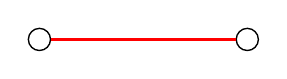
\begin{tikzpicture}[scale=0.66]

\GraphInit[vstyle=Simple]

\SetUpEdge[lw = 1.1pt, color = red]
\tikzset{VertexStyle/.append style = {minimum size = 8pt, inner sep = 0pt, fill=white}}    

\Vertices[unit=2]{circle}{1,2}

\Edges(1,2)

\end{tikzpicture}
\end{inparaenum}

\item {\bf n = 3}

\begin{inparaenum}
\item 
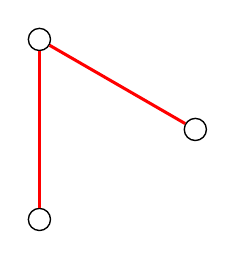
\begin{tikzpicture}[scale=0.66]

\GraphInit[vstyle=Simple]

\SetUpEdge[lw = 1.1pt, color = red]
\tikzset{VertexStyle/.append style = {minimum size = 8pt, inner sep = 0pt, fill=white}}    

\Vertices[unit=2]{circle}{1,2,3}

\Edges(1,2,3)

\end{tikzpicture}
\qquad\item
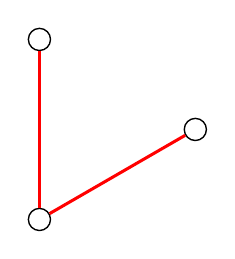
\begin{tikzpicture}[scale=0.66]

\GraphInit[vstyle=Simple]

\SetUpEdge[lw = 1.1pt, color = red]
\tikzset{VertexStyle/.append style = {minimum size = 8pt, inner sep = 0pt, fill=white}}    

\Vertices[unit=2]{circle}{1,2,3}

\Edges(1,3,2)

\end{tikzpicture}
\qquad\item
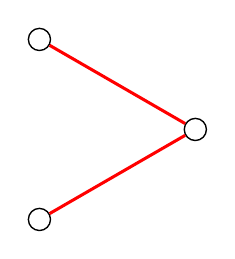
\begin{tikzpicture}[scale=0.66]

\GraphInit[vstyle=Simple]

\SetUpEdge[lw = 1.1pt, color = red]
\tikzset{VertexStyle/.append style = {minimum size = 8pt, inner sep = 0pt, fill=white}}    

\Vertices[unit=2]{circle}{1,2,3}

\Edges(2,1,3)

\end{tikzpicture}
\end{inparaenum}

\item {\bf n = 4}

\begin{inparaenum}
\item
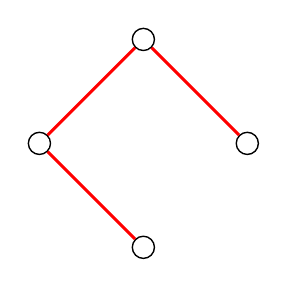
\begin{tikzpicture}[scale=0.66]

\GraphInit[vstyle=Simple]

\SetUpEdge[lw = 1.1pt, color = red]
\tikzset{VertexStyle/.append style = {minimum size = 8pt, inner sep = 0pt, fill=white}}    

\Vertices[unit=2]{circle}{1,2,3,4}

\Edges(1,2,3,4)

\end{tikzpicture}
\item
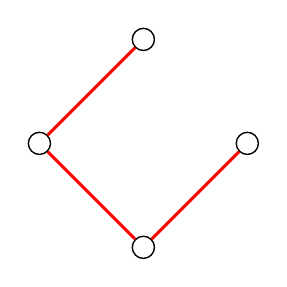
\begin{tikzpicture}[scale=0.66]

\GraphInit[vstyle=Simple]

\SetUpEdge[lw = 1.1pt, color = red]
\tikzset{VertexStyle/.append style = {minimum size = 8pt, inner sep = 0pt, fill=white}}    

\Vertices[unit=2]{circle}{1,2,3,4}

\Edges(2,3,4,1)

\end{tikzpicture}
\item
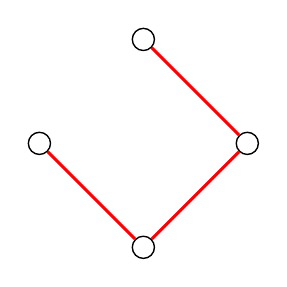
\begin{tikzpicture}[scale=0.66]

\GraphInit[vstyle=Simple]

\SetUpEdge[lw = 1.1pt, color = red]
\tikzset{VertexStyle/.append style = {minimum size = 8pt, inner sep = 0pt, fill=white}}    

\Vertices[unit=2]{circle}{1,2,3,4}

\Edges(3,4,1,2)

\end{tikzpicture}
\item
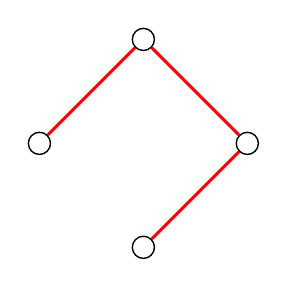
\begin{tikzpicture}[scale=0.66]

\GraphInit[vstyle=Simple]

\SetUpEdge[lw = 1.1pt, color = red]
\tikzset{VertexStyle/.append style = {minimum size = 8pt, inner sep = 0pt, fill=white}}    

\Vertices[unit=2]{circle}{1,2,3,4}

\Edges(4,1,2,3)

\end{tikzpicture}
\end{inparaenum}

\begin{inparaenum}
\item[5.]
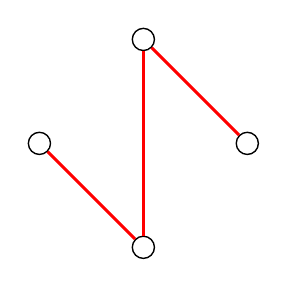
\begin{tikzpicture}[scale=0.66]

\GraphInit[vstyle=Simple]

\SetUpEdge[lw = 1.1pt, color = red]
\tikzset{VertexStyle/.append style = {minimum size = 8pt, inner sep = 0pt, fill=white}}    

\Vertices[unit=2]{circle}{1,2,3,4}

\Edges(1,2,4,3)

\end{tikzpicture}
\item[6.]
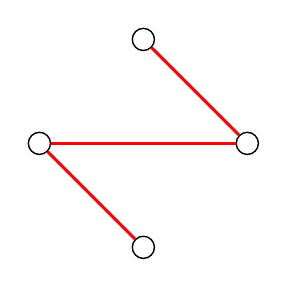
\begin{tikzpicture}[scale=0.66]

\GraphInit[vstyle=Simple]

\SetUpEdge[lw = 1.1pt, color = red]
\tikzset{VertexStyle/.append style = {minimum size = 8pt, inner sep = 0pt, fill=white}}    

\Vertices[unit=2]{circle}{1,2,3,4}

\Edges(2,1,3,4)

\end{tikzpicture}
\item[7.]
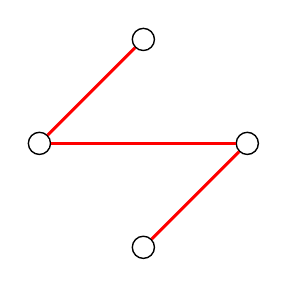
\begin{tikzpicture}[scale=0.66]

\GraphInit[vstyle=Simple]

\SetUpEdge[lw = 1.1pt, color = red]
\tikzset{VertexStyle/.append style = {minimum size = 8pt, inner sep = 0pt, fill=white}}    

\Vertices[unit=2]{circle}{1,2,3,4}

\Edges(2,3,1,4)

\end{tikzpicture}
\item[8.]
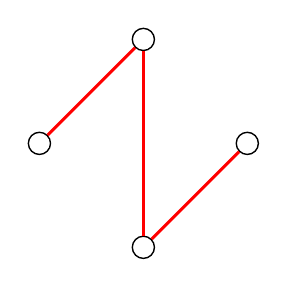
\begin{tikzpicture}[scale=0.66]

\GraphInit[vstyle=Simple]

\SetUpEdge[lw = 1.1pt, color = red]
\tikzset{VertexStyle/.append style = {minimum size = 8pt, inner sep = 0pt, fill=white}}    

\Vertices[unit=2]{circle}{1,2,3,4}

\Edges(3,2,4,1)

\end{tikzpicture}

\end{inparaenum}

\end{itemize}



\end{document}